The following analysis is performed on data generated using the reconstruction techniques described above, choosing the best of all three ${E}_{\gamma}$ solutions, with  ${m}_{\gamma} = {m}_{\nu} = 0$. Unless otherwise explicitly stated, the beam background removal was not cheated but the lorentz boost into the centre of mass frame was performed. The analysis was conducted considering only the muon signal of the data set, as this is the focus of this analysis.
\\\\

%---------------------------------------------------------------------------------------------------------------------------------------------------------%---------------------------------------------------------------------------------------------------------------------------------------------------------
\subsection{Cut Flow}
\label{SUBSEC:CutFlow}

All the same cuts as in Ivan’s thesis \cite{IvanMarchesini} were sequentially applied to obtain a cut flow histogram, which tests the efficiency of each of the cuts. The results of this analysis were then compared to Ivan's to see how it is performing. Further, the flow diagram was created again by cheating the beam background removal, and by applying the additional initial cut that the ISR energy is small (${E}_{\gamma}^{MC} < 1$ GeV). The final plot was made to see if the ISR made a considerable contribution to the efficiency of the cuts.
\\\\
There are a few subtle differences between the cuts that Ivan and the cuts made in this analysis, due to the reconstruction methods each implemented. The first was the cut on the jet reconstruction variables ${y}_{+}$ and ${y}_{-}$. In this analysis FastJets was forced to reconstruct two jets, corresponding to the 2 quarks, and physically this is the minimum number of jets that can occur, as single quark cannot be created. This means the cut on the ${y}_{-}$ variable that Ivan makes is unphysical in this analysis. Ivan applies this cut because he also considered final states with 4 quarks. The lepton cut that was made here make is also different to Ivan’s. The IsolatedLeptonTaggingProcessor was used, so the implemented cut was that a single isolated lepton is reconstructed. There are a considerable number of events where the processor reconstructed zero particles, and so this cut can be significant. Ivan on the other hand used a jet reconstruction processor with a specific energy cut to reconstruct isolated leptons. The final difference is that Ivan makes a 'charged lepton' cut, which is not described in his thesis. A similar cut is not made in this analysis and so the corresponding efficiency will not change across this cut.
\\\\
For convenience the cuts and efficiencies are tabulated in Table.~\ref{TAB:SelectionEfficiencies}, and the resulting total flow diagram can be seen in (Figure.~\ref{FIG:Flow}).
\\\\
\begin{table}[!]
    \centering
    \caption{
        Selection efficiency of sequantially applied cuts. Where the post ISR correction ${m}_{W}^{lep}$ was calculated using all 3 possible ${E}_{\gamma}$ solutions. (*) Indicates cuts where the current and Ivan's cuts differ, as discussed in the text.
    }
    \resizebox{0.8\textwidth}{!}{%
    \begin{tabular}{|l|l|l|l|l|l|} \hline
        Order & Cut description & \multicolumn{4}{c|}{Efficiency [\%]} \\ \cline{3-6}
        & & \multicolumn{3}{c|}{My Results} & Ivan's Results \\  \cline{3-5}
        & & n = 2129 & \multicolumn{2}{c|}{n = 99419} & n = 107233 \\ \cline{4-5}
        & & & no cheat & cheat & \\ \hline \hline
        0 & muon signal & 100.00 & 100.00 & 100.00 & 100.00 \\ \hline
        1 & track multiplicity\tablefootnote{track mulitplicity was taken as the number of reconstructed charged particles.} ${n}_{tracks} \ge 10$ & 97.13 & 97.01 & 96.23 & 99.996 \\ \hline
        2 & center of mass energy $\sqrt{s} > 100$ GeV & 92.29 & 91.69 & 84.35 & 97.96 \\ \hline
        3 & total transverse momentum ${P}_{T} > 5$ GeV & 91.16 & 90.47 & 83.28 & 96.69 \\ \hline
        4 & total energy ${E}_{SUM} < 500$ GeV & 89.66 & 89.28 & 82.70 & 95.36 \\ \hline
        5 & $\ln{({y}_{+})} \in [-12, -3]$ (*) & 88.69 & 88.08 & 82.47 & 95.01 \\ \hline
        6 & 1 lepton found (*) & 80.65 & 80.77 & 81.50 & 78.75 \\ \hline
        7 & pre ISR correction ${m}_{W}^{lep} \in [20, 250]$ GeV &  78.23 & 77.94 & 77.84 & 76.61 \\ \hline
        8 & tau discrimination\tablefootnote{${\tau}_{discr}$ defined by ${\tau}_{discr} = {(\frac{2{E}_{lep}}{\sqrt{s}})}^{2} + {(\frac{{m}_{W}^{lep}}{{m}_{W}^{true}})}^{2}$} &  76.05 & 75.60 & 75.73 & 74.07 \\ \hline
        9 & charged lepton (*) & 76.05 & 75.60 & 75.73 & 73.51 \\ \hline
        10 & isolation variable\tablefootnote{$\Delta{\Omega}_{iso}$ defined as,
        \begin{align}
            ({\phi}_{lep} - {\phi}_{had}) < \pi \to \Delta{\Omega}_{iso} &= \sqrt{{({\theta}_{lep} - {\theta}_{had})}^{2}+{({\phi}_{lep} - {\phi}_{had})}^{2}} \\
            ({\phi}_{lep} - {\phi}_{had}) \ge \pi \to \Delta{\Omega}_{iso} &= \sqrt{{({\theta}_{lep} - {\theta}_{had})}^{2} + {(2\pi - |{\phi}_{lep} - {\phi}_{had} |)}^{2}} \, .
        \end{align}} ${\Delta\Omega}_{iso} > 0.5$ & 76.01 & 75.58 & 75.72 & 73.42 \\ \hline
        11 & post ISR correction ${m}_{W}^{lep} \in [40, 120]$ GeV & 72.90 & 72.77 & 72.33 & 70.13 \\ \hline
        12 & post ISR correction ${m}_{W}^{had} \in [40, 120]$ GeV & 63.21 & 62.92 & 70.52 & 66.93 \\ \hline
        13 & $\cos{{\theta}_{W}} > -0.95$ & 63.02 & 62.65 & 70.21 & 66.78 \\ \hline
        \end{tabular}
        }
        \label{TAB:SelectionEfficiencies}
    \end{table}

\begin{figure}[!]
    \centering
    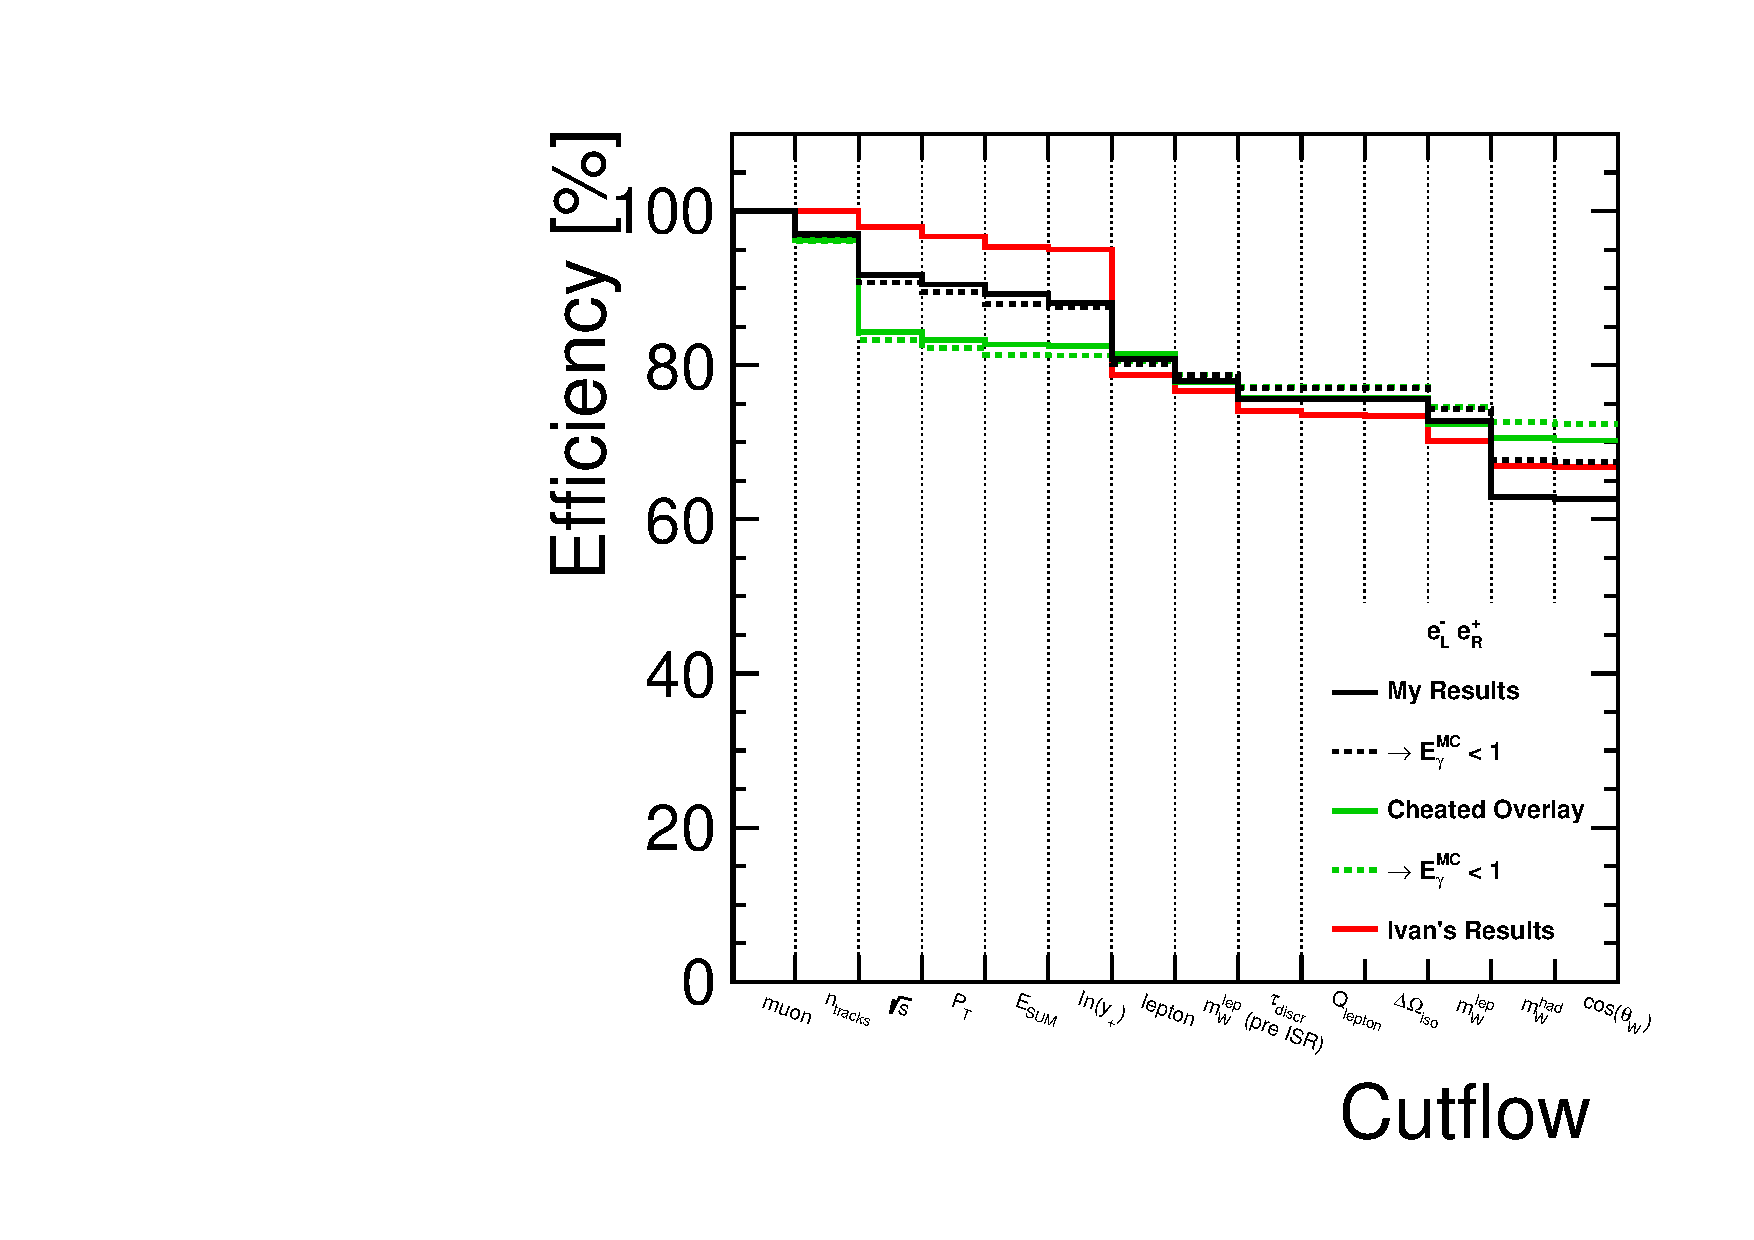
\includegraphics[width=0.8\textwidth]{\imagepath/P_HistFlow3_All.pdf}
    \caption{
    Cut flows comparing the results of this analysis (with and whithout cheating overlay removal) to previous studies.  The results of this analysis considering a signal where ${E}_{\gamma} < 1$ are also displayed. The cuts on the x axis are as defined in Table.~\ref{TAB:SelectionEfficiencies}.
    }
    \label{FIG:Flow}
\end{figure}

There is a considerable difference in the cut efficiencies before the 'lepton' cut. In all of the events where no isolated leptons are reconstructed, the leptonic W boson is reconstructed entiely from the invisble neutrino, will be completely wrong. The efficiency of the cheated and un-cheated background removal reconstructions converge on this lepton cut, suggesting that the differences observed before the cut are due to these incorrectly reconstructed events. When this lepton cut is applied to the current results before the rest of the cuts, the large discrepancy is not observed, providing support to this hypothesis (see Appendix.~\ref{HistFLowIsolep}).
\\\\
After the lepton cut, the efficiency of the reconstruction is higher than in previous studies, until the cut on the ${m}_{W}^{had}$ where it is considerably worse. By looking at the cheated results though, which don't drop in efficiency as dramatically, it can be suggested that this is due to the performsnce of the beam background removal process. Further, after the lepton cut the ${E}_{\gamma}^{MC} < 1$ GeV signal is consistently performing better than the full signal, which suggests that large ISR energies reduces the efficiency of the reconstruciton and so the detector.

%---------------------------------------------------------------------------------------------------------------------------------------------------------%---------------------------------------------------------------------------------------------------------------------------------------------------------
\subsection{Angle Cut Efficiencies}
\label{SUBSEC:AngleCutEfficiencies}
In this section the final result of the analysis, to evaluate the angular dependancy of the cut efficiency, is discussed. The efficiency was obtained for both the full signal and the ${E}_{\gamma}^{MC} < 1$ GeV signal, the results of which are shown in Figure.~\ref{FIG:AngleEfficiencies}.
\\
\begin{figure}
    \begin{subfigure}[t]{0.32\textwidth}
        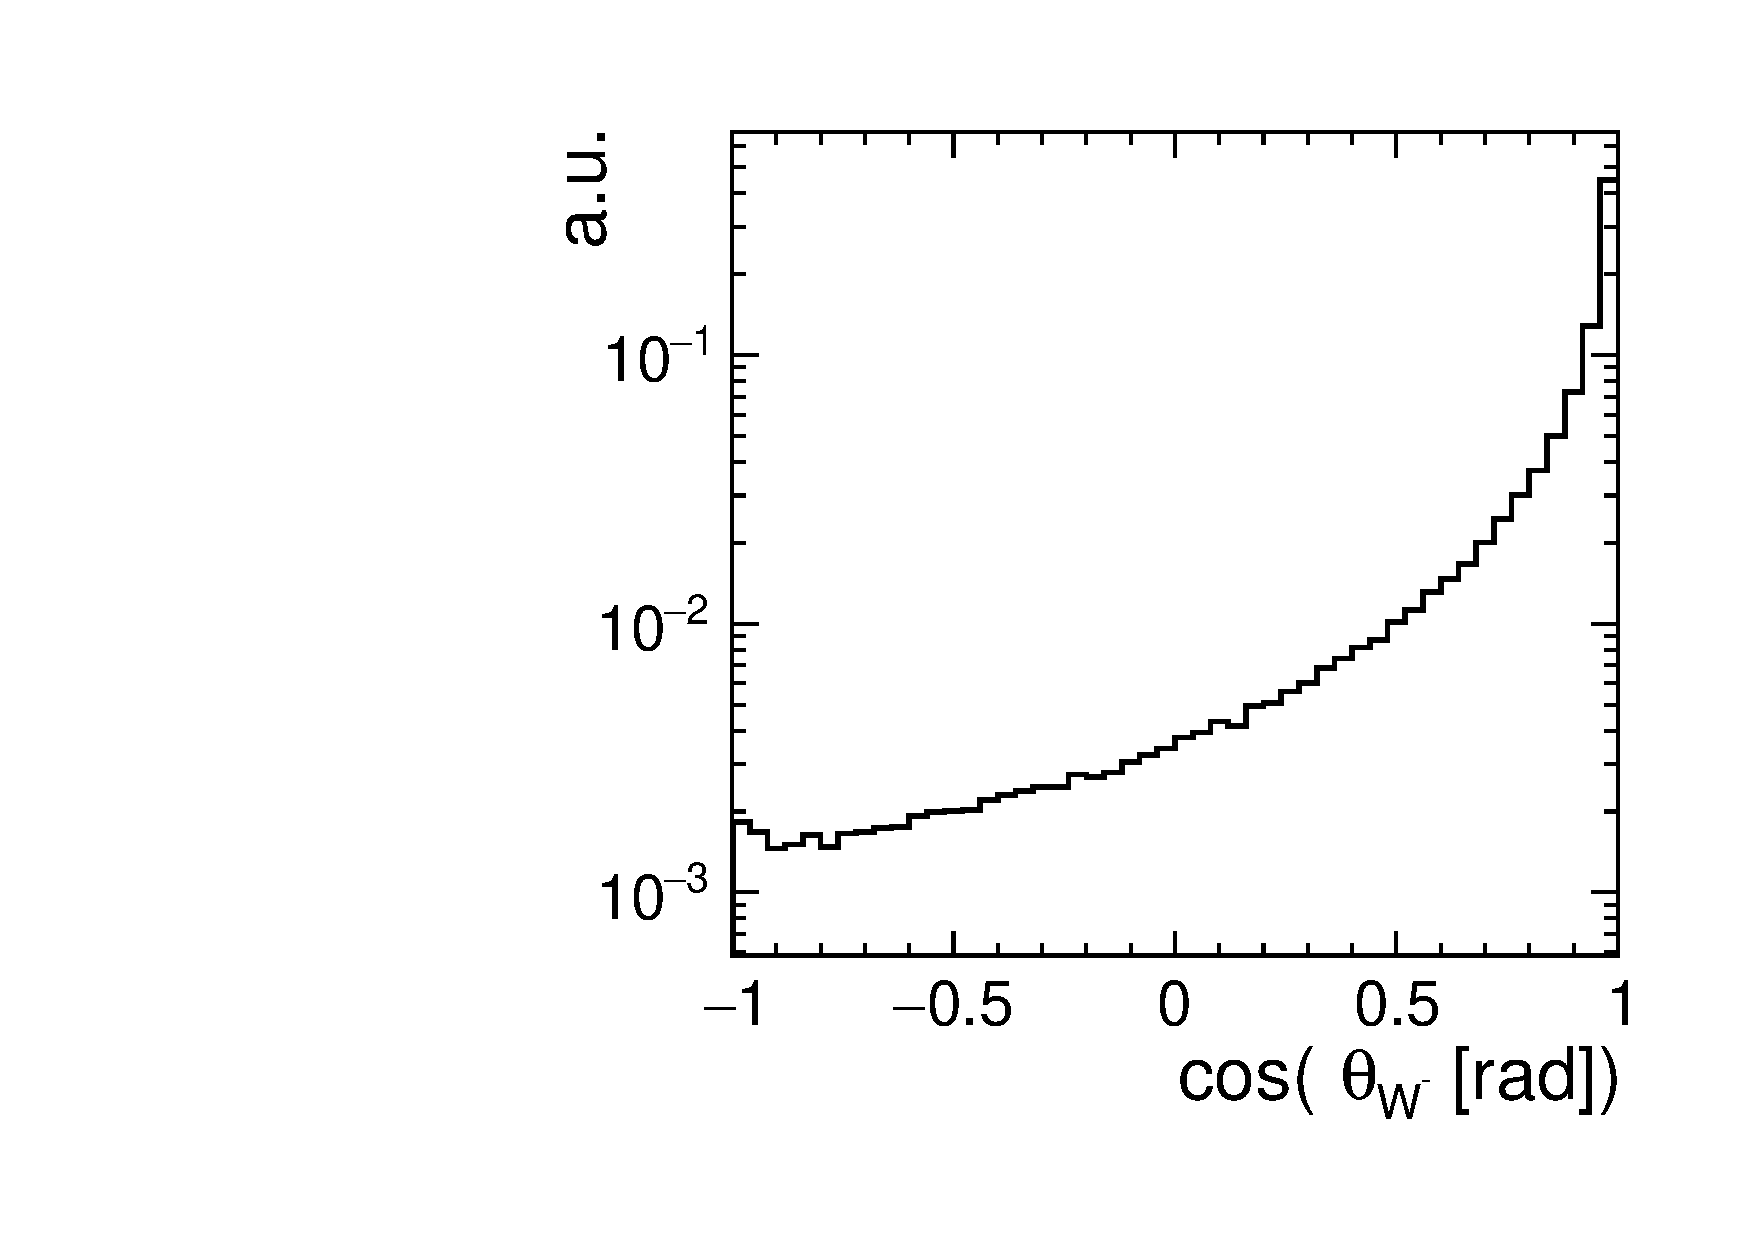
\includegraphics[width=\textwidth]{\imagepath/ThetaMin_cos.pdf}
        \caption{}
        \label{SUBFIG:ThetaMin}
    \end{subfigure}
    \begin{subfigure}[t]{0.32\textwidth}
        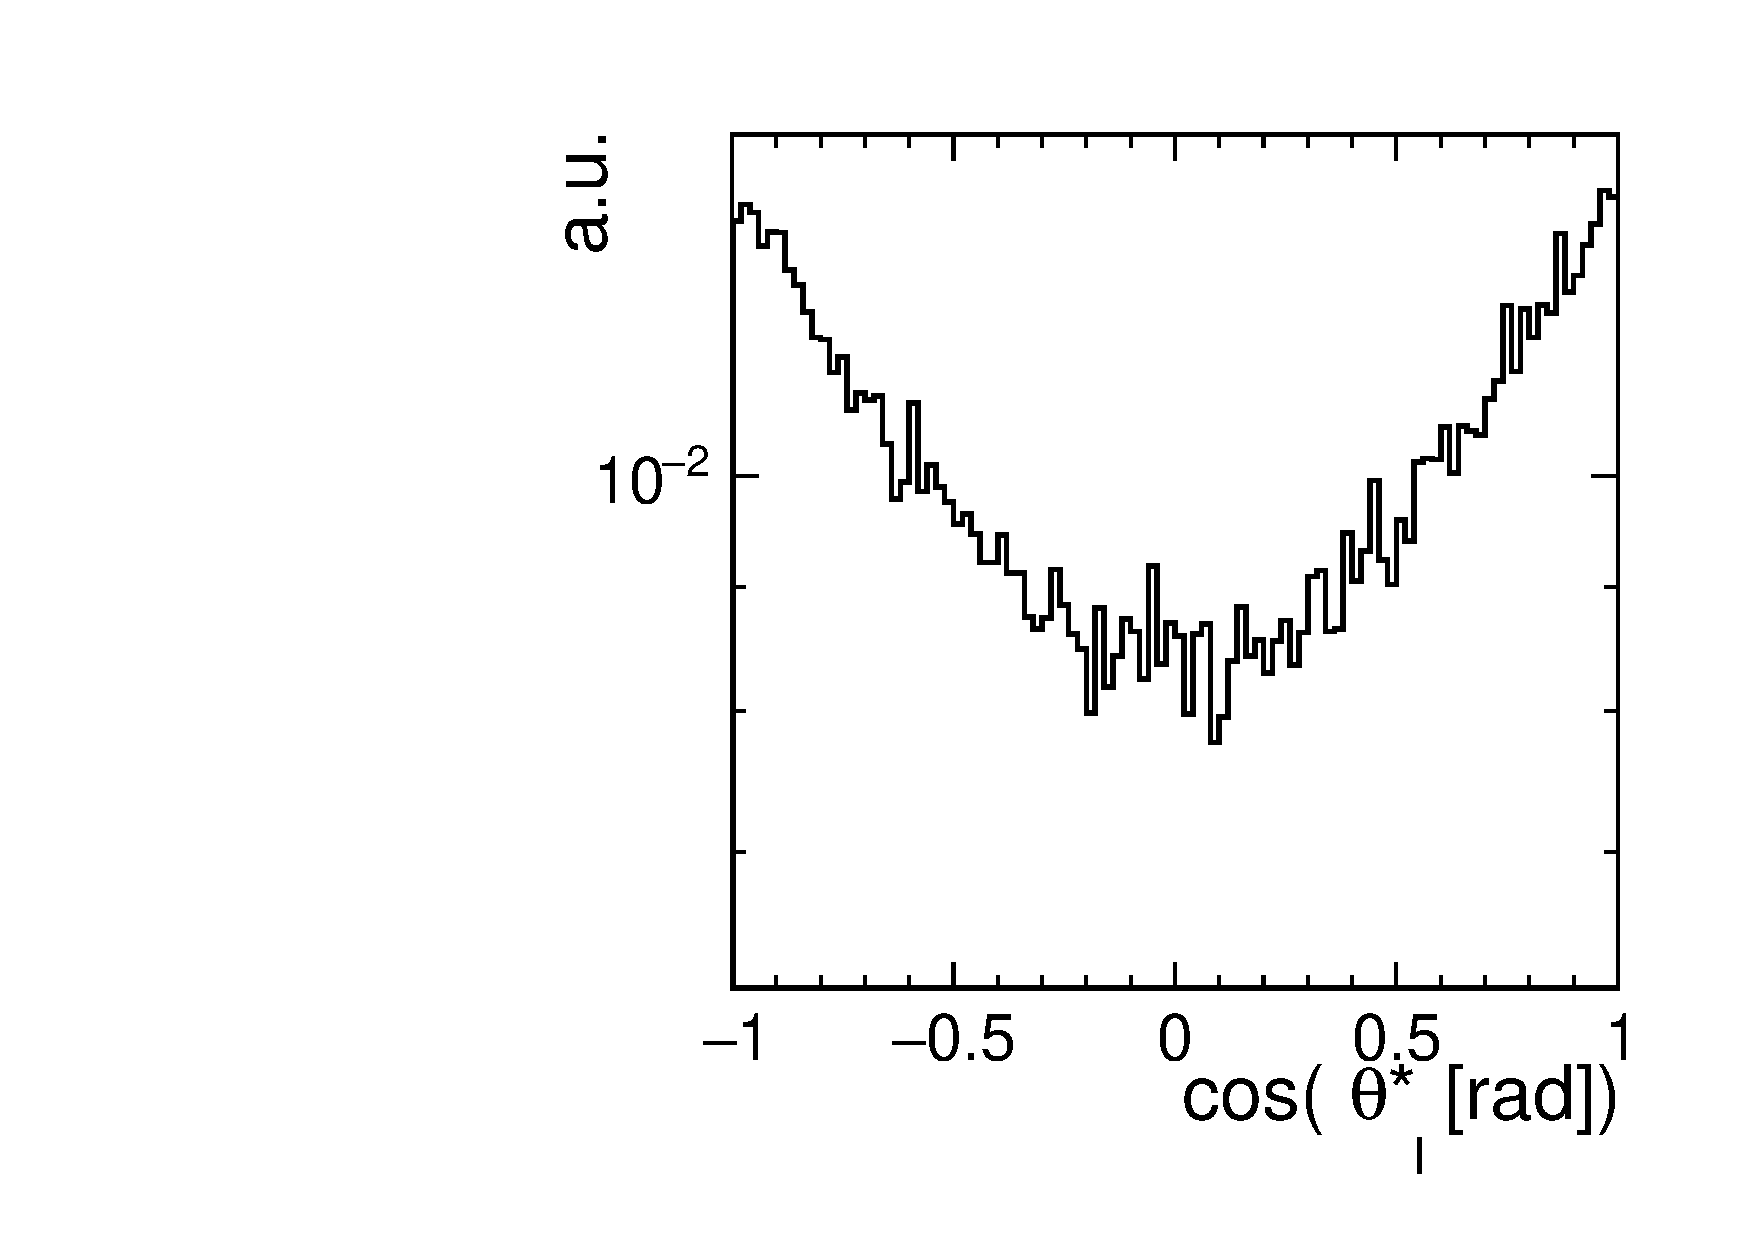
\includegraphics[width=\textwidth]{\imagepath/ThetaLep_cos.pdf}
        \caption{}
        \label{SUBFIG:ThetaLep}
    \end{subfigure}
    \begin{subfigure}[t]{0.32\textwidth}
        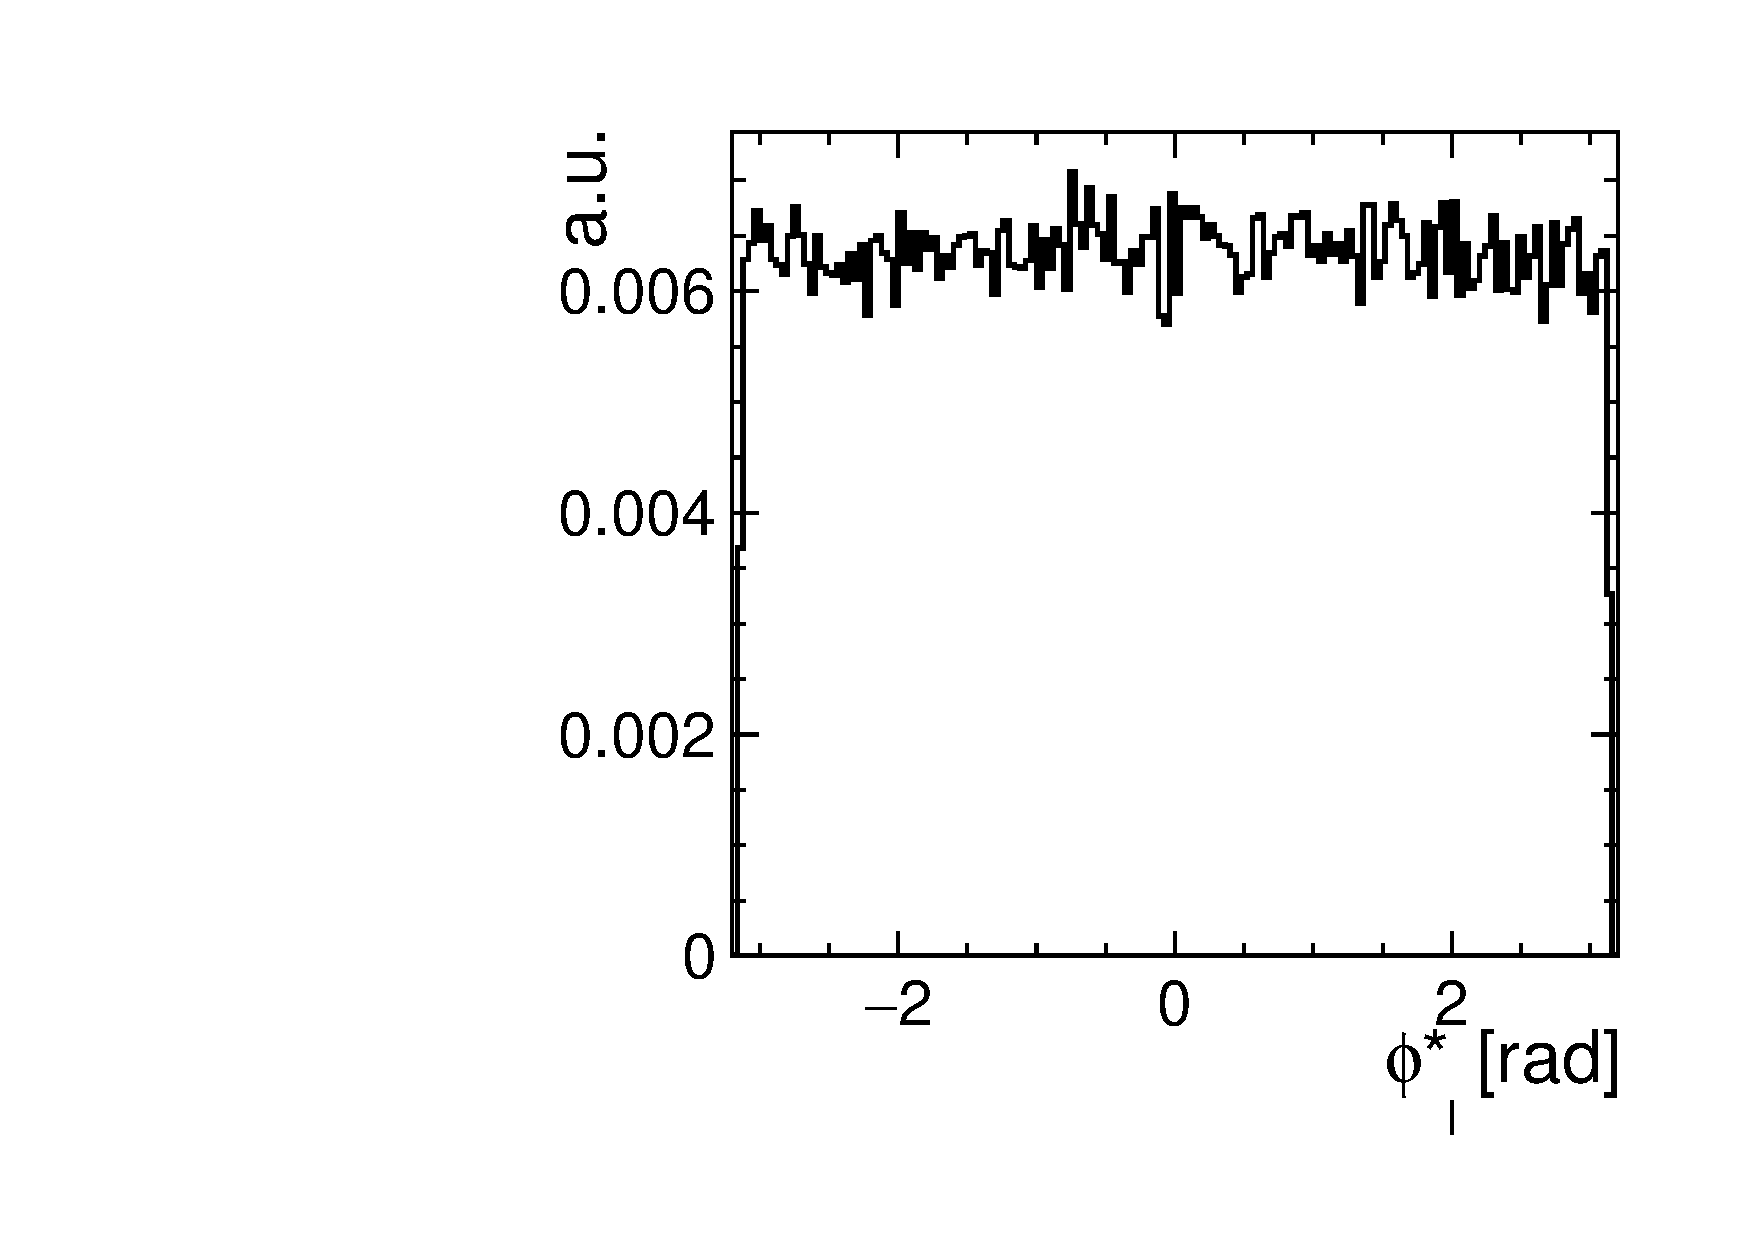
\includegraphics[width=\textwidth]{\imagepath/PhiLep.pdf}
        \caption{}
        \label{SUBFIG:PhiLep}
    \end{subfigure}\\
    \begin{subfigure}[t]{0.32\textwidth}
        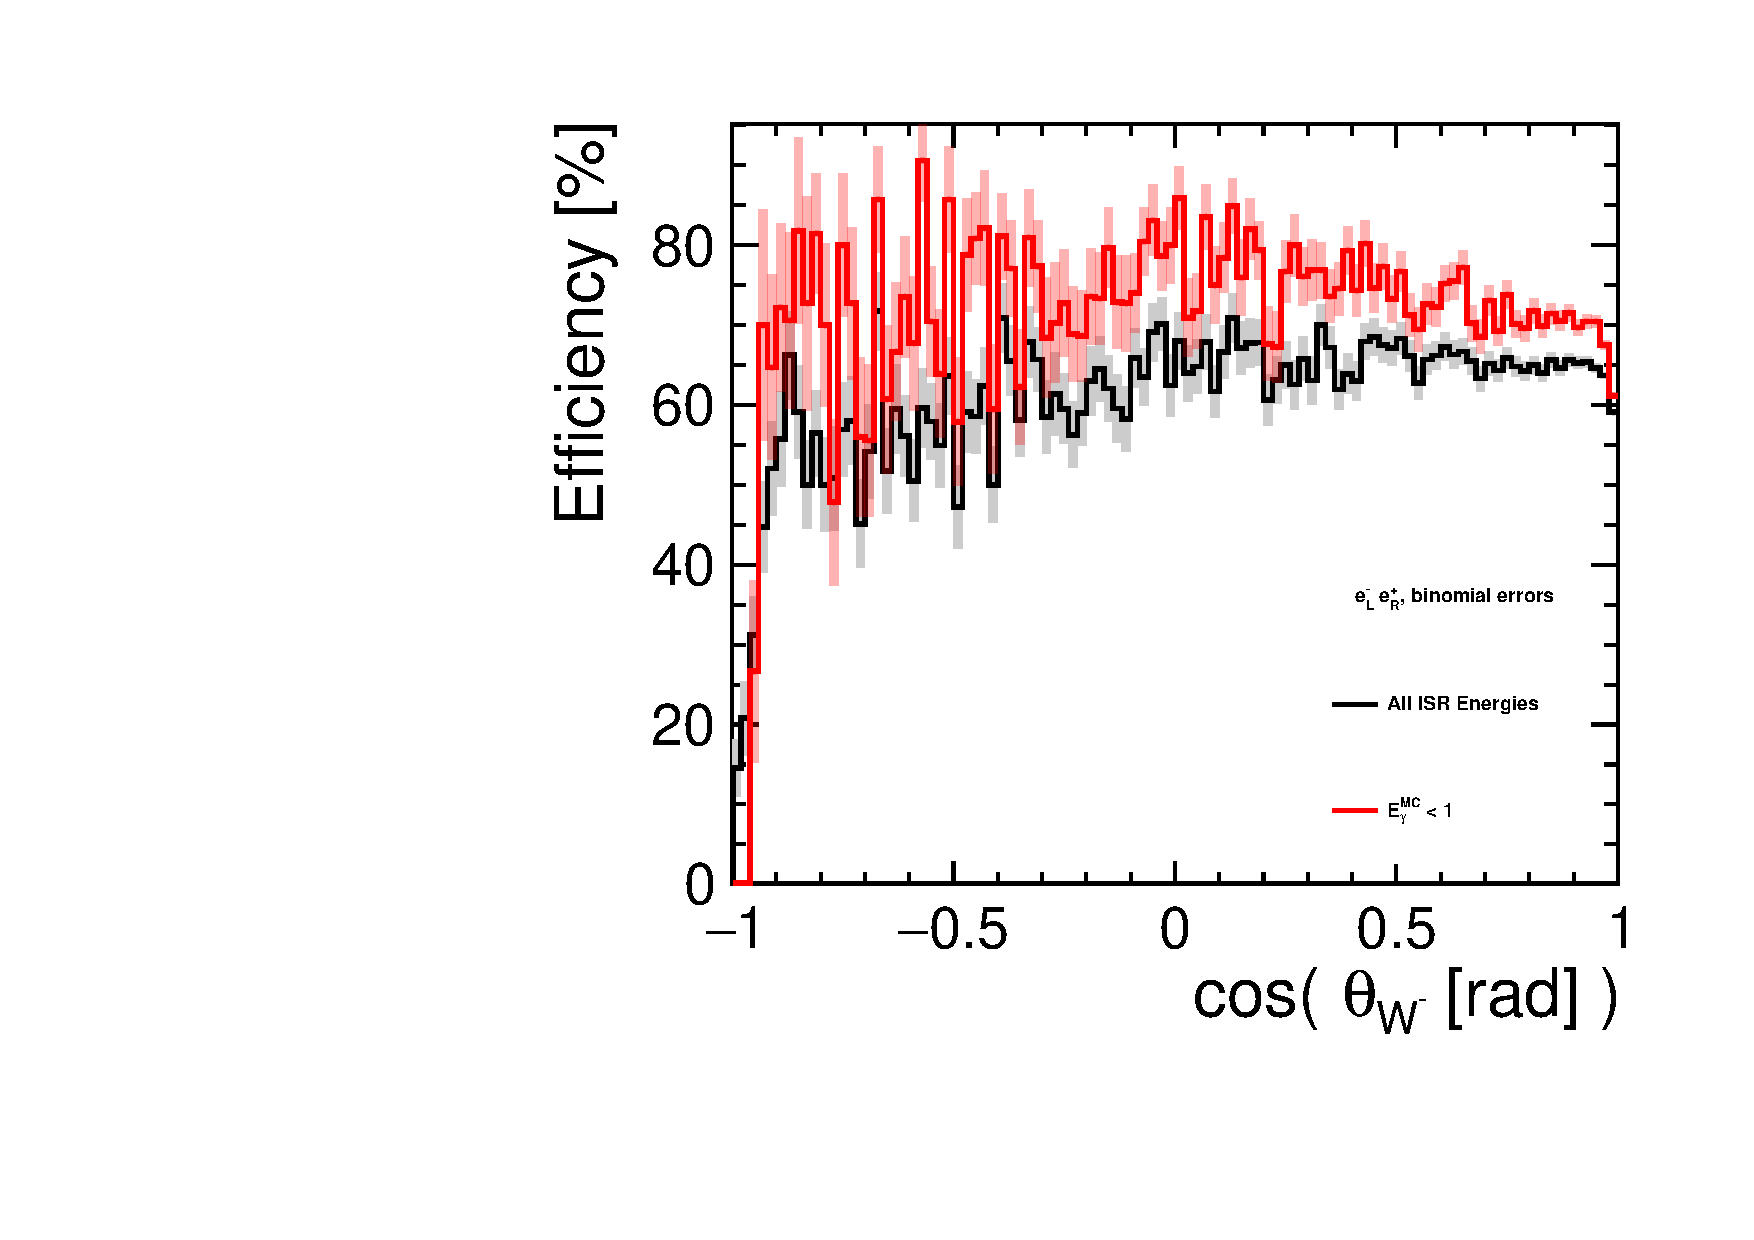
\includegraphics[width=\textwidth]{\imagepath/P_E_ThetaMin_cos_err_Both.pdf}
        \caption{}
        \label{SUBFIG:ThetaMinError}
    \end{subfigure}
    \begin{subfigure}[t]{0.32\textwidth}
        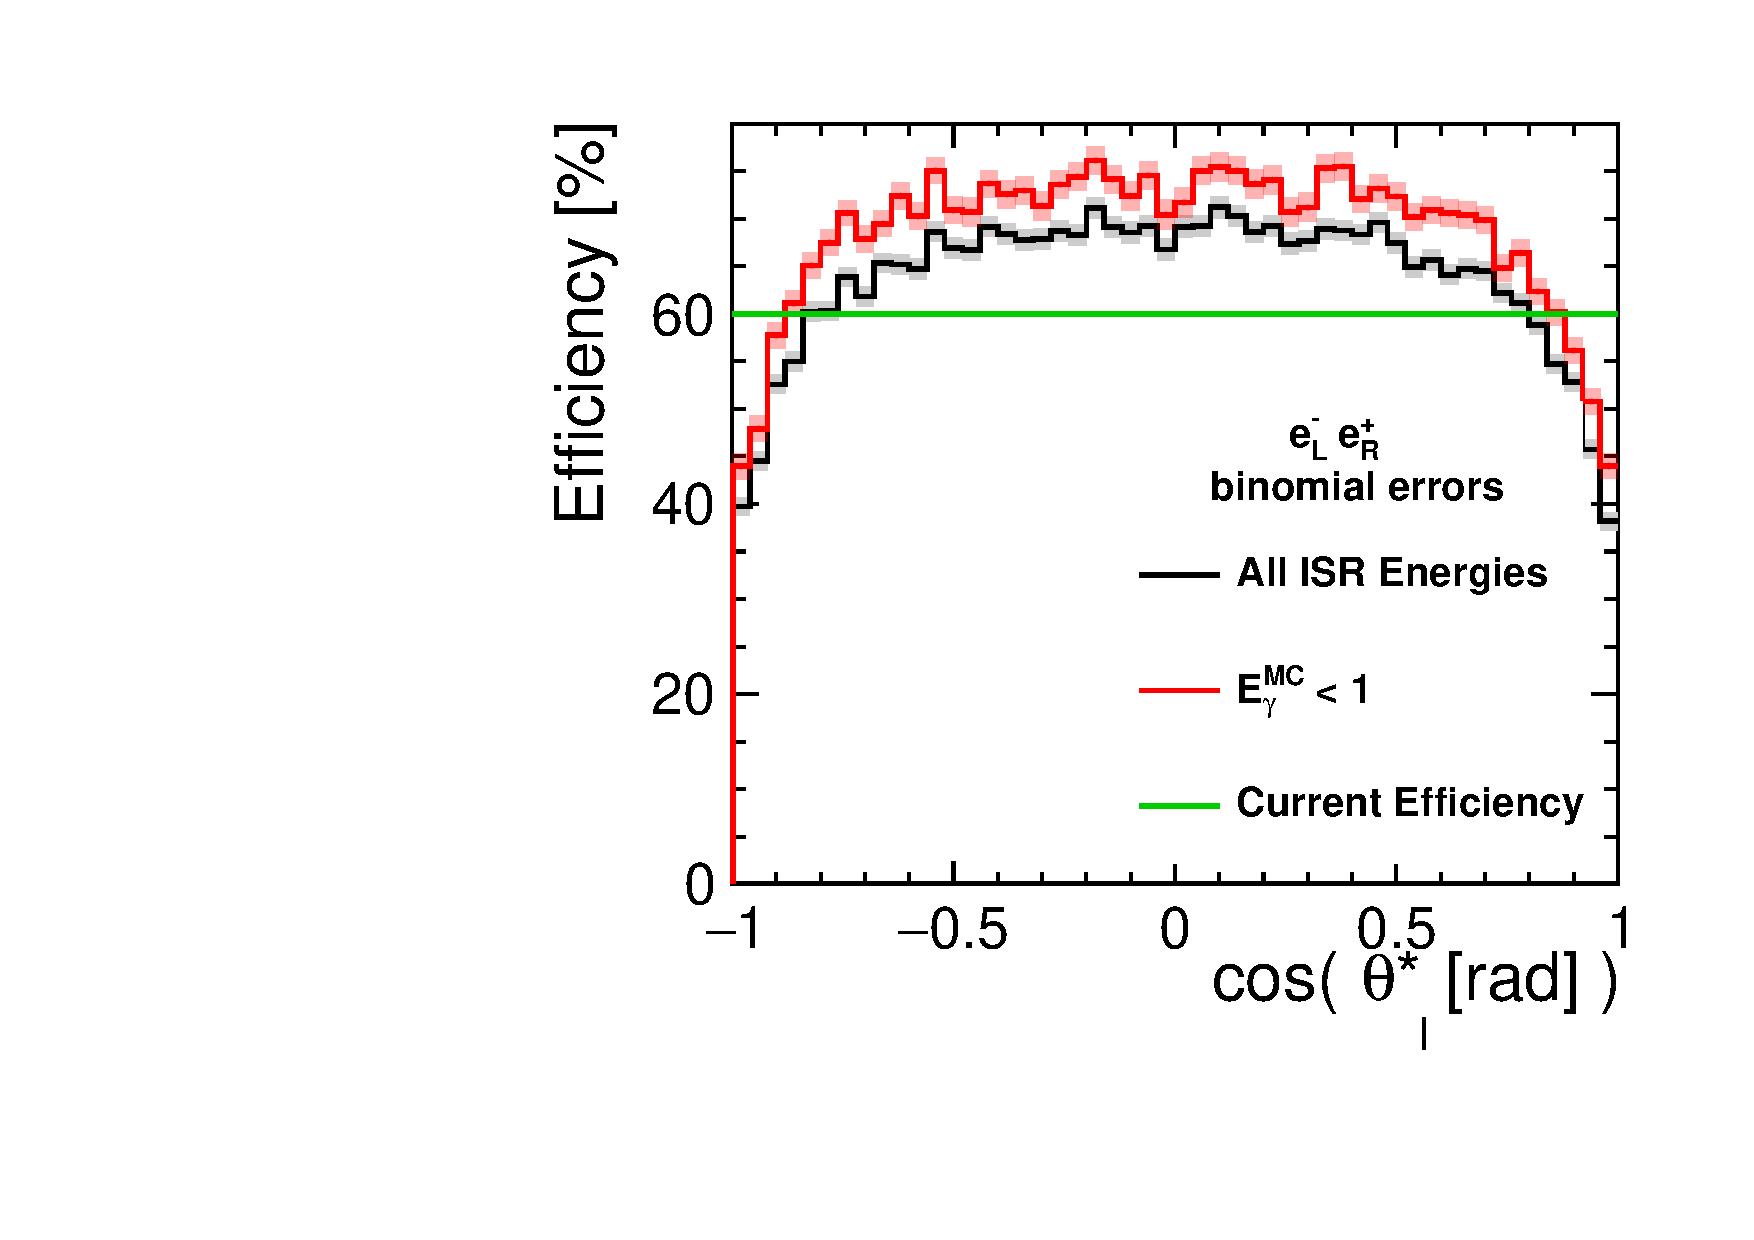
\includegraphics[width=\textwidth]{\imagepath/P_E_ThetaLep_cos_err_Both.pdf}
        \caption{}
        \label{SUBFIG:ThetaLepError}
    \end{subfigure}
    \begin{subfigure}[t]{0.32\textwidth}
        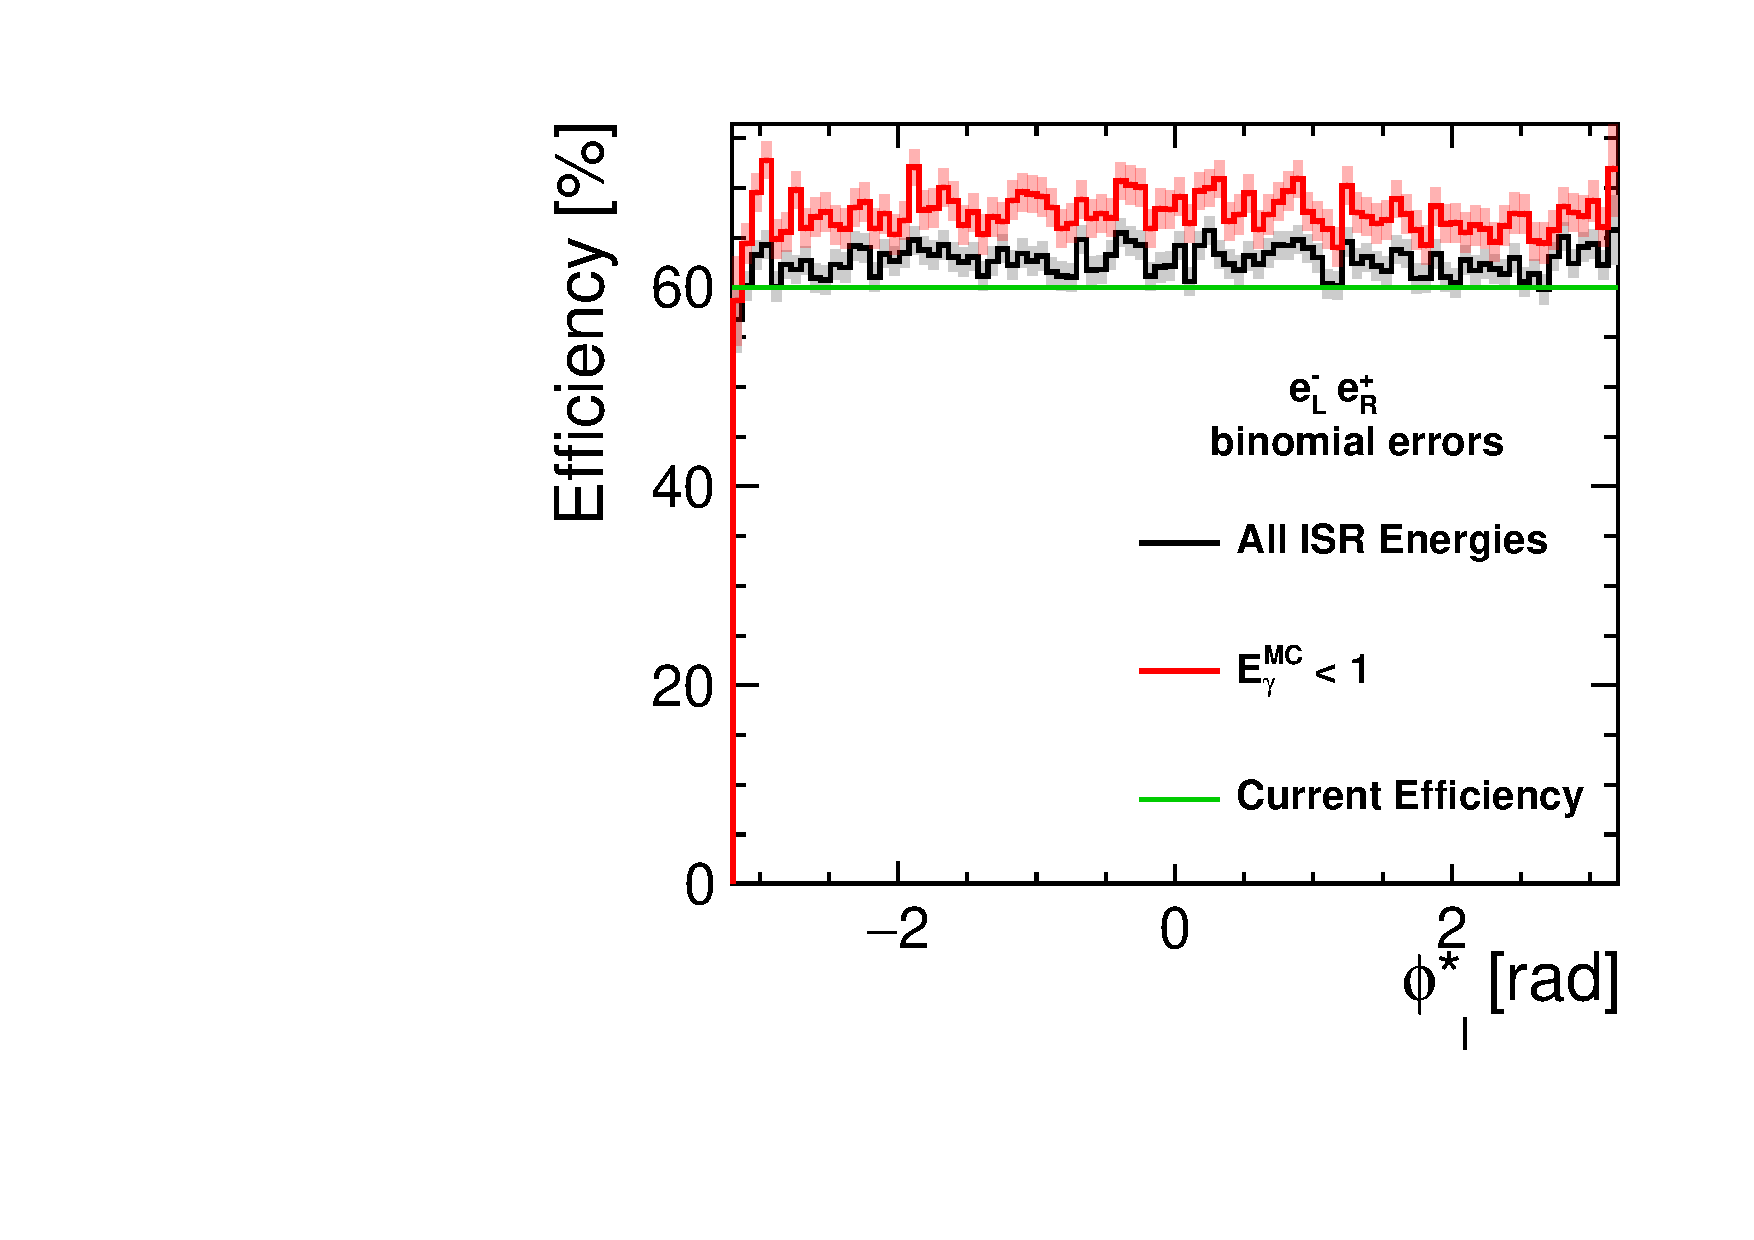
\includegraphics[width=\textwidth]{\imagepath/P_E_PhiLep_err_Both.pdf}
        \caption{}
        \label{SUBFIG:PhiLepError}
    \end{subfigure}
    \caption{
    \subfigref{SUBFIG:ThetaMin}, \subfigref{SUBFIG:ThetaLep} and \subfigref{SUBFIG:PhiLep} are the extracted angles as defined in Figure.~\ref{FIG:Angles}. \\
    \subfigref{SUBFIG:ThetaMinError}, \subfigref{SUBFIG:ThetaLepError} and \subfigref{SUBFIG:PhiLepError} are the associated cut efficiencies, after applying the cuts outlined in Table.~\ref{TAB:SelectionEfficiencies}.
    }
    \label{FIG:AngleEfficiencies}
\end{figure}

The $\cos{({\theta}_{{W}^{-}})}$ distribution is statistically limited towards -1, in the backwards direction, greatly reducing the efficiency. Due to the low mass of the neutrino, it becomes more virtual as more momentum is trasnferred to it, reducing the cross section. As a result most of the momentum transfer is to the W bosons, aligning it to the lepton it decayed from. In this case the ${W}^{-}$ momentum is preferably aligned to the momentum of the ${e}^{-}$ and so we see the angular distribution is highly biased towards the $\cos{({\theta}_{{W}^{-}})} = 1$ side. It is, however, reasonably constant throughout the rest of the distribution. The efficiency has a clear angular dependance on $\cos{({\theta}_{l}^{*})}$, with lower efficiency in regions closely aligned to the beam-pipe. Due to the coordinate system used this is not trivially explained, however for W bosons highly aligned to the beam pipe, the lepton appears to decay in a preferably transverse direction in the center of mass frame of such a boson. The ${\phi}_{l}^{*}$ of efficiency has a uniform efficiency as well as angular distribution, somewhat expected due to the uniformity of the W bosons ${\phi}$ distribution.
\\\\
The ${E}_{\gamma}^{MC} < 1$ GeV signal has a higher efficiency than the full signal, but the angular dependance as a similar form. The magnitude of the efficiency differs by a constant factor.
